This appendix describes a repeat experiment similar to the conditions in Chapter \ref{chap5}. A repeat experiment was performed to show the uniformity of temperature distribution on the surface, therefore justifying the reason of placement for the representative thermocouples shown in Figure \ref{fig:thermocouple}

\subsection*{About Experimental Conditions}
A repeat experiment was performed on April 29-30, 2026. This is around one month after the experiment in Chapter \ref{chap5} was conducted on March 11-12, 2026.

As will be seen in the next section, the exact temperature distribution in \ref{fig:18} will not be seen. These are due to the ambient temperature conditions which are difficult to control and maintain as the experiments are performed:
\begin{itemize}
\item Number of people in the laboratory.
\item Air conditioner settings (which were kept constant as much as possible).
\item The weather for the day.
\item Season of measurement: it is generally warmer outside in April compared to March.
\item Long hours of experiment: ambient temperature throughout the day cannot be kept constant or controlled.
\end{itemize}

The thermocouple placement for the repeat experiment is as shown in Figure \ref{fig:thermocouple_repeat}. Once again, the thermocouples were placed on the centers of their respective surface. Compared to Figure \ref{fig:thermocouple} however, two more sensors were added: $T_\mathrm{top,out,1}$ and $T_\mathrm{top,out,3}$ to fully characterize the top surface of the transformer ferrite core. The thermocouple $T_\mathrm{top,out,2}$ represents the center of the top surface, similar to Figure \ref{fig:thermocouple}.

\begin{figure}[h!]
    \centering
        \includegraphics[width=0.85\columnwidth]{figures_chapter5/thermocouple.pdf}%
    \caption{Thermocouple placement for the measurement of key spots in the transformers. Thermocouples  $T_{\mathrm{left, out}}$, and $T_{\mathrm{bot, out}}$ are placed on the center of their respective faces as well. $T_\mathrm{top,out,1}$ and $T_\mathrm{top,out,3}$. $T_\mathrm{top, out, 2}$ represents the center of the top surface, similar to Figure \ref{fig:thermocouple}.}
    \label{fig:thermocouple_repeat}
\end{figure}

\subsection*{Experimental Results}
The measured temperature profiles of the edgewise and flatwise transformers during natural cooling are shown in Figure~\ref{fig:repeat}a and Figure~\ref{fig:repeat}b respectively. The temperature profiles of the edgewise and flatwise transformers during forced-air cooling are shown in Figure~\ref{fig:repeat}c and Figure~\ref{fig:repeat}d respectively. In natural cooling, a steady-state $T_{\mathrm{wind}}$ of 76.0$^{\circ}$C and 70.8$^{\circ}$C were observed for the edgewise-wound and flatwise-wound transformer respectively. In forced-air cooling, a steady-state $T_{\mathrm{wind}}$ of 42.0$^{\circ}$C and 37.4$^{\circ}$C were observed for the edgewise-wound and flatwise-wound transformer respectively. Both transformers seemed to reach their steady-state temperatures at the same speed.

The key internal-to-external gradients observed in both cooling conditions for both transformers have differences with what has been observed in Chapter \ref{chap5} due to the reasons explained in the previous section. But,more importantly, the main benefit of the flatwise-wound configuration as seen in Chapter \ref{chap5} is still seen in this repeat experiment.

More importantly, as for the aims of this repeat experiment, the transformers designed can operate in extended time duration without failure. It can also be noted that the differences in the temperature between  $T_\mathrm{top,out,1}$, $T_\mathrm{top,out,2}$, and  $T_\mathrm{top, out, 3}$ are not that significant. Small differences may only be caused by equipment errors and tolerances. Therefore, taking from the middle part of each face is suitable to avoid parasitic thermal resistances affecting the temperature measurement spots.

\begin{figure}[H]
\centering
% (a) Left circuit
        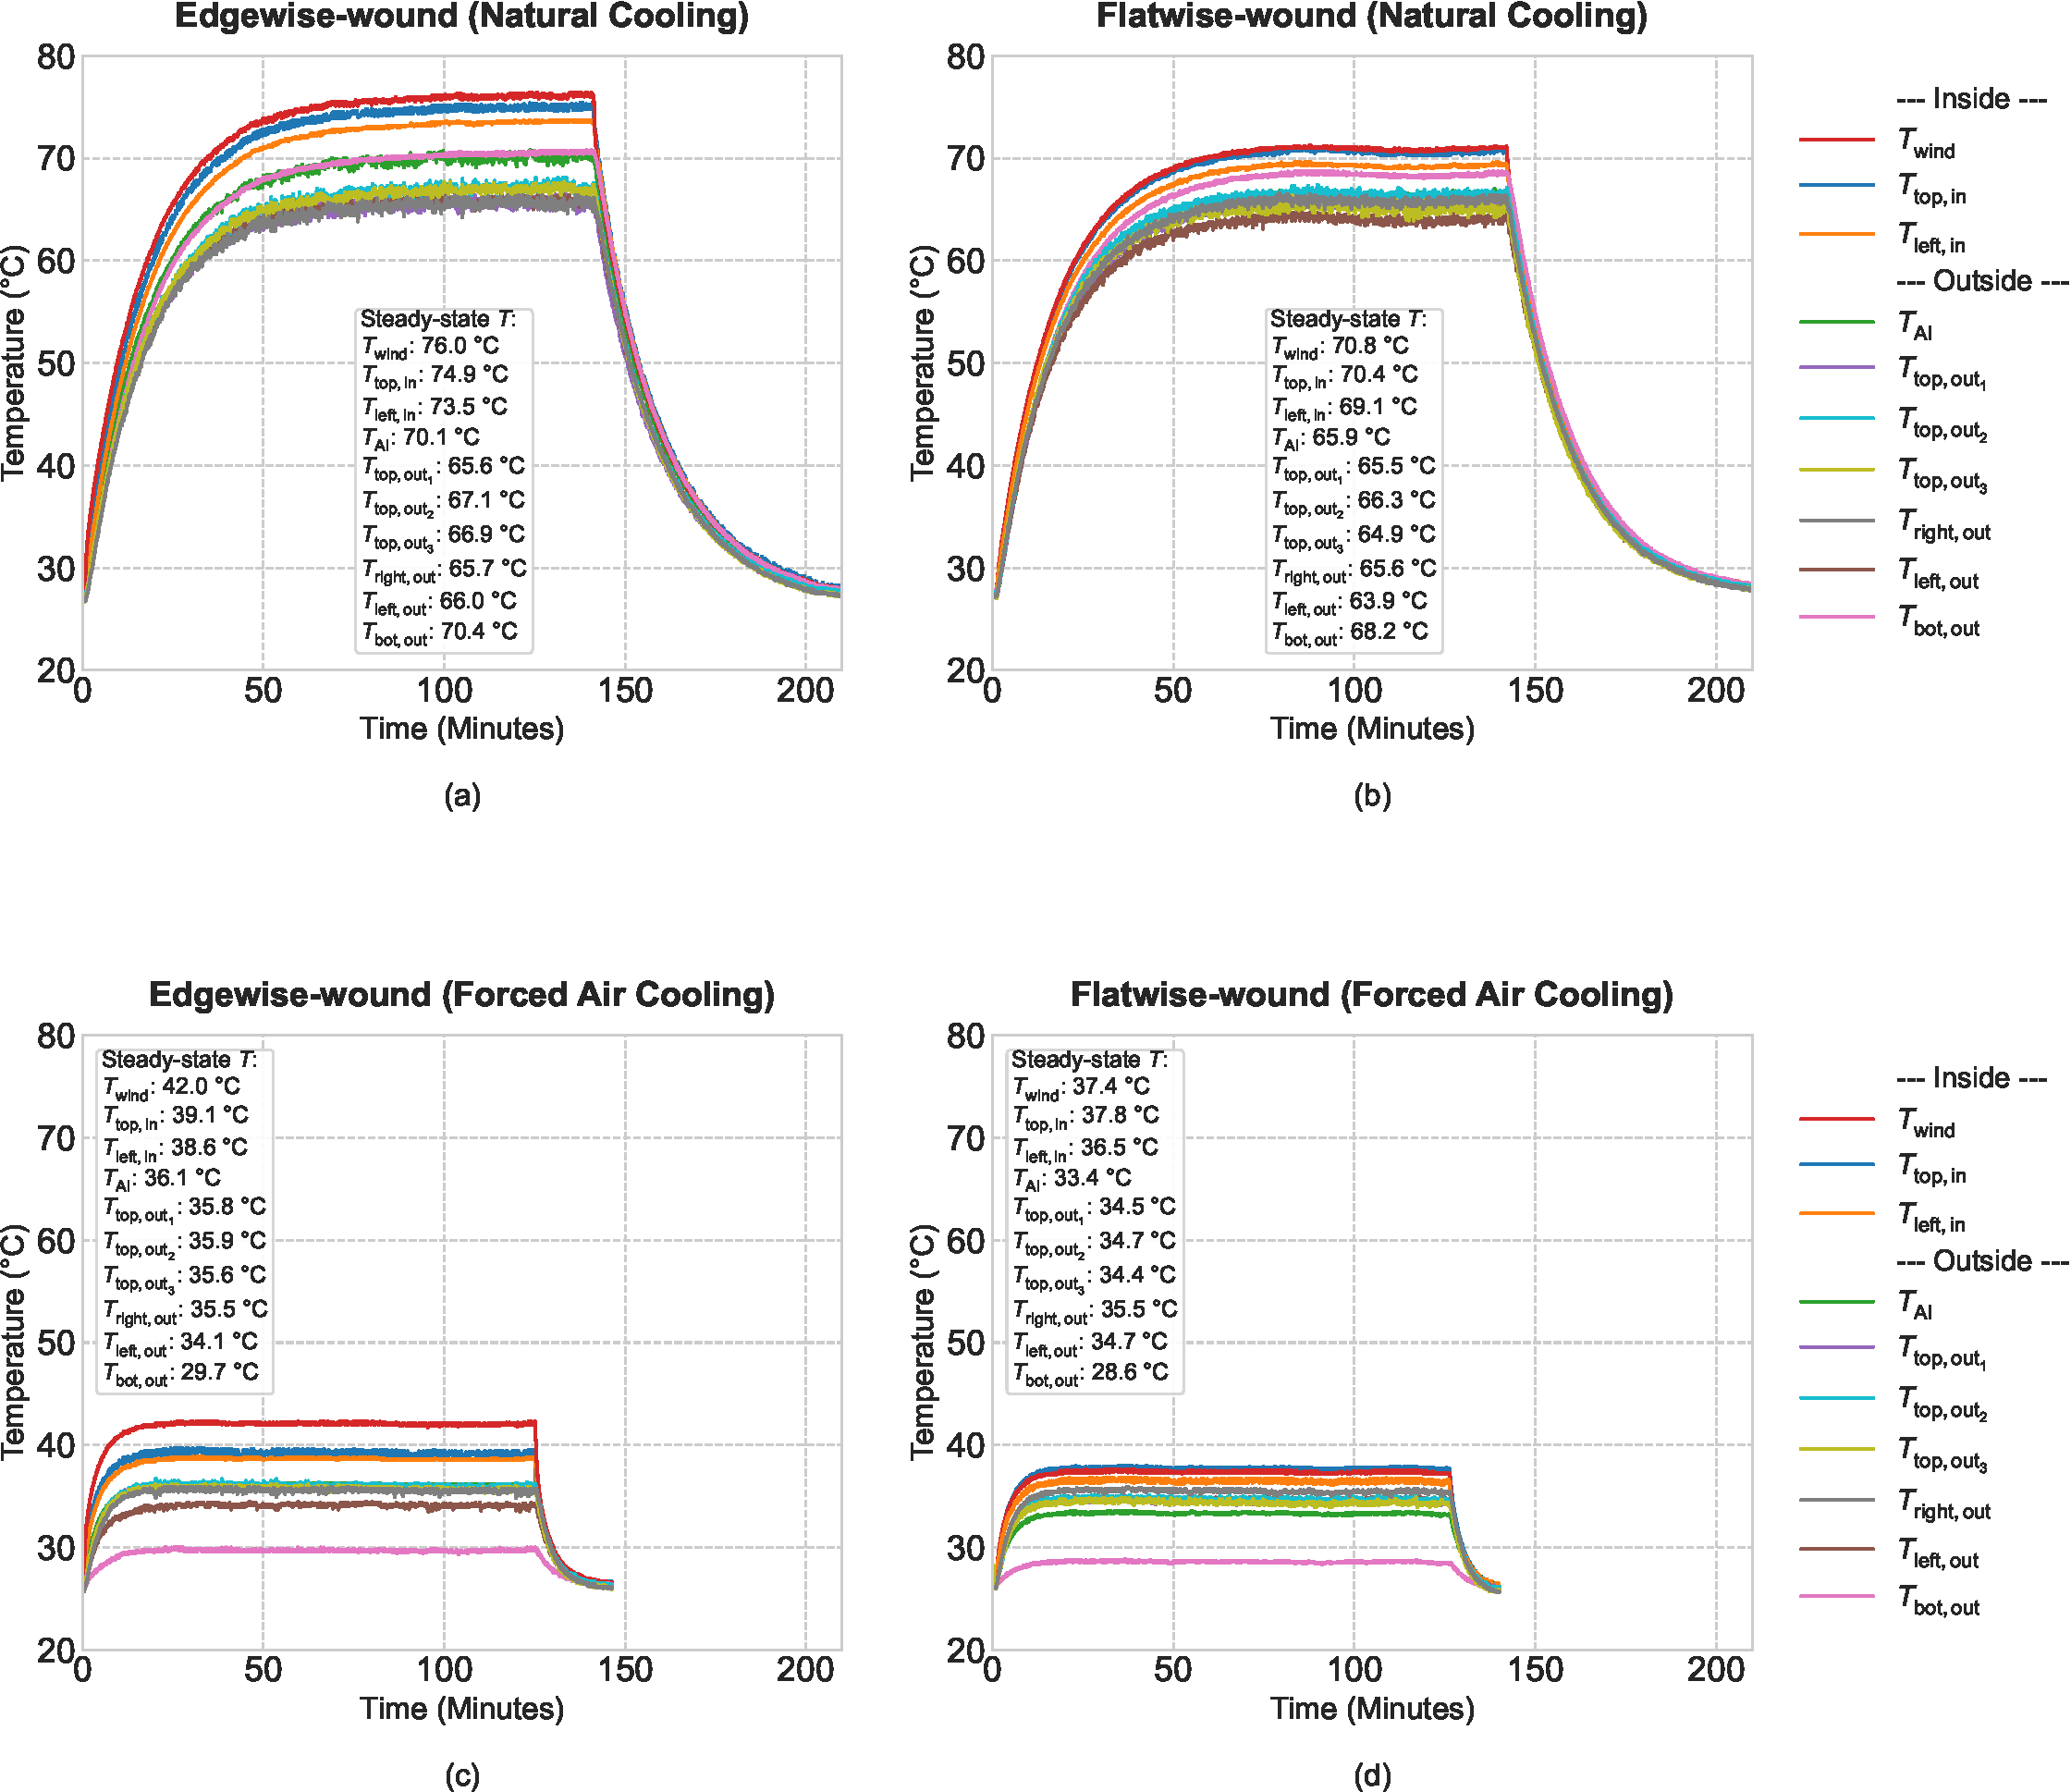
\includegraphics[width=\columnwidth]{images/Combined_Thermal_Comparison.pdf} 
        \caption{Temperature profiles of the transformers at natural cooling: (a) edgewise-wound transformer, (b) flatwise-wound transformer; and forced-air cooling through a heat sink: (c) edgewise-wound transformer, (d) flatwise-wound transformer.}
        \label{fig:repeat}
\end{figure}